% Standalone vector inset designed for the 43%-width method minipage.
% The analytic surface and seed locations match the earlier schematic,
% with horizontal coordinates rescaled to the normalised action box.
\documentclass[border=2pt]{standalone}
\usepackage{times}
\usepackage[T1]{fontenc}
\usepackage{tikz,pgfplots}
\usetikzlibrary{arrows.meta,decorations.markings,shapes.geometric}
\pgfplotsset{compat=1.18}
% Central colour palette shared by the paper and all active figures.
% Method colours identify methods, not dataset conditions or phases.
\def\PaperPaletteLoaded{1}

% Paper-wide method and neutral colours.
\definecolor{paperCorePivot}{HTML}{008577}
\definecolor{paperCorePivotLight}{HTML}{E5F3EF}
\definecolor{paperIQL}{HTML}{3F6C8E}
\definecolor{paperTD3BC}{HTML}{8A681F}
\definecolor{paperCalQL}{HTML}{397C70}
\definecolor{paperBC}{HTML}{7654A3}
\definecolor{paperBCLight}{HTML}{F0EBF7}
\definecolor{paperPD}{HTML}{303030}
\definecolor{paperNeutralLight}{HTML}{F7F8F9}
\definecolor{paperReference}{HTML}{183B65}
\definecolor{paperInk}{HTML}{202B35}
\definecolor{paperGray}{HTML}{7A8286}
\definecolor{paperBackground}{HTML}{F9FAFB}
\definecolor{paperGrid}{HTML}{BFC3C6}
\definecolor{paperSummary}{HTML}{565656}
\definecolor{paperBand}{HTML}{777777}
\definecolor{paperSilver}{HTML}{AEB4BC}
\definecolor{paperSilverLight}{HTML}{EDF0F3}
\definecolor{paperSilverEdge}{HTML}{626A73}
\definecolor{paperPropellerLight}{HTML}{E4EEF7}
\definecolor{paperPropellerEdge}{HTML}{3974A1}

% Semantic aliases used by the framework overview.
\colorlet{hmBehavior}{paperBC}%
\colorlet{hmInk}{paperInk}%
\colorlet{hmGray}{paperGray}%
\colorlet{hmPaper}{paperBackground}%
\colorlet{overviewPolicyEdge}{paperCorePivot}%
\colorlet{overviewPolicyFill}{paperCorePivot!25}%
\colorlet{overviewActionEdge}{paperInk!70}%
\colorlet{overviewActionOuterFill}{paperGray!20}%
\colorlet{overviewDPEdge}{paperInk}%
\colorlet{overviewDPFill}{paperPropellerLight}%
\colorlet{droneAccent}{paperSilver}%
\colorlet{droneLight}{paperSilverLight}%

% Dataset-construction figure colours.
\definecolor{hdBlue}{RGB}{0,114,178}
\definecolor{hdPurple}{RGB}{145,94,155}
\definecolor{hdGood}{RGB}{0,130,115}
\definecolor{hdMedium}{RGB}{216,155,38}
\definecolor{hdBad}{RGB}{185,80,77}
\definecolor{hdInk}{RGB}{45,52,64}
\definecolor{hdPaper}{RGB}{248,250,252}

% Legacy illustration names retained for compatibility with optional figures.
\definecolor{policyedge}{RGB}{203,55,111}
\definecolor{policycoreedge}{RGB}{215,50,32}
\definecolor{policyfill}{RGB}{233,198,213}
\definecolor{policycorefill}{RGB}{236,196,199}
\definecolor{actionedge}{RGB}{61,77,150}
\definecolor{actionfill}{RGB}{159,154,199}
\definecolor{actionouterfill}{RGB}{159,208,240}
\definecolor{actoredge}{RGB}{155,77,152}
\definecolor{dpedge}{RGB}{7,10,28}
\definecolor{dpfill}{RGB}{227,228,233}
\definecolor{hmBlue}{RGB}{0,114,178}%

% Shared critic-landscape colour map.
\pgfplotsset{
  colormap={referencecriticmap}{
    color(0cm)=(paperCorePivot!5)
    color(1cm)=(paperCorePivot!22)
    color(2cm)=(paperCorePivot!65)
  }
}

\begin{document}
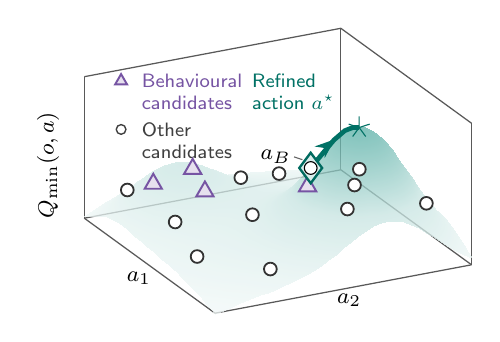
\begin{tikzpicture}
\tikzset{declare function={
 q(\x,\y)=1.15*exp(-((1.5*\x-0.85)^2+(1.5*\y-0.55)^2)/0.5)
 +0.42*exp(-((1.5*\x+0.9)^2+(1.5*\y+0.75)^2)/0.38)
 -0.08*((1.5*\x)^2+(1.5*\y)^2);
}}
\begin{axis}[
 width=6.5cm,height=5.2cm,view={63}{37},
 domain=-1:1,y domain=-1:1,samples=35,samples y=35,
 xmin=-1,xmax=1,ymin=-1,ymax=1,zmin=-.35,zmax=1.18,
 point meta min=-.36,point meta max=1.07076,
 colormap name=referencecriticmap,
 xlabel={$a_1$},ylabel={$a_2$},
 label style={font=\fontsize{8}{9}\selectfont,inner sep=1pt},
 xtick=\empty,ytick=\empty,ztick=\empty,
 axis line style={black!65,line width=.45pt},
 axis background/.style={fill=white},clip=false,
]
\addplot3[surf,shader=interp,z buffer=sort,opacity=.75,draw=none]
 {q(x,y)};
\addplot3[only marks,mark=*,mark size=2.3pt,
 draw=black!80,fill=white,line width=.65pt] coordinates {
 (-.80000,-.76667,-.00346) (-.83333,.43333,-.15688)
 (-.63333,.03333,.00611) (-.33333,.76667,-.11116)
 (-.13333,-.73333,-.01565) (.13333,-.26667,.07785)
 (.33333,-.80000,-.13181) (.80000,-.46667,-.11485)
 (.86667,.10000,.41997) (.76667,.76667,.25596)
 (.13333,.56667,.35164) (.21333,.14667,.51602)
 };
\addplot3[only marks,mark=triangle*,mark size=3.6pt,
 draw=paperBC,fill=paperBC!18,line width=.7pt] coordinates {
 (-.48000,-.42000,.29862) (-.20000,.33333,.05672)
 (-.26667,-.43333,.16812) (-.53333,-.70000,.18345)
 };
\draw[paperCorePivot!85!black,line width=1.7pt,
 postaction={decorate},decoration={markings,
 mark=at position .57 with {\arrow{Stealth[length=2.5mm,width=1.9mm]}}}]
 (axis cs:.21333,.14667,.51602) --
 (axis cs:.29333,.20000,.70262) --
 (axis cs:.37333,.24667,.87499) --
 (axis cs:.44667,.29333,1.00069) --
 (axis cs:.50667,.32667,1.05799) --
 (axis cs:.54757,.35431,1.07076);
\addplot3[only marks,mark=diamond*,mark size=5.5pt,
 draw=paperCorePivot!80!black,fill=paperCorePivot!15,line width=.85pt]
 coordinates {(.21333,.14667,.51602)};
\addplot3[only marks,mark=*,mark size=2.3pt,draw=black,fill=white]
 coordinates {(.21333,.14667,.51602)};
\addplot3[only marks,mark=star,mark size=4pt,
 draw=paperCorePivot!85!black,fill=paperCorePivot!85!black]
 coordinates {(.54757,.35431,1.07076)};
% Direct labels replace the tiny three-item legend and footer sentence.
\node[font=\sffamily\fontsize{7}{8}\selectfont,
 text=paperBC,anchor=north west,align=left,inner sep=1pt,fill=none]
 at (axis description cs:.14,.85)
 {Behavioural\\candidates};
\node[draw=paperBC,fill=paperBC!18,regular polygon,
 regular polygon sides=3,minimum size=5pt,inner sep=0pt,line width=.7pt]
 at (axis description cs:.095,.815) {};
\node[font=\fontsize{8}{9}\selectfont,anchor=east,inner sep=1pt]
 at ([xshift=-6pt,yshift=4pt]axis cs:.21333,.14667,.51602) {$a_B$};
\draw[black!60,line width=.4pt]
 ([xshift=-6pt,yshift=4pt]axis cs:.21333,.14667,.51602)
 -- ([xshift=-3pt,yshift=3pt]axis cs:.21333,.14667,.51602);
\node[font=\sffamily\fontsize{7}{8}\selectfont,
 text=paperCorePivot!85!black,anchor=north west,inner sep=1pt,align=left,fill=none]
 at (axis description cs:.425,.85)
 {Refined\\action $a^\star$};
\node[font=\sffamily\fontsize{7}{8}\selectfont,
 text=black!75,anchor=north west,inner sep=1pt,align=left,fill=none]
 at (axis description cs:.14,.68)
 {Other\\candidates};
\node[circle,draw=black!75,fill=none,minimum size=3.5pt,
 inner sep=0pt,line width=.5pt]
 at (axis description cs:.095,.645) {};
\node[rotate=90,font=\fontsize{8}{9}\selectfont,anchor=south]
 at (axis description cs:-.04,.52) {$Q_{\min}(o,a)$};
\end{axis}
\end{tikzpicture}
\end{document}
